\section{Analiza sistema}

Student pravi profil gde popunjava osnovne podatke o sebi, bira oblasti interesovanja i postavlja dodatne filtere. Na osnovu izabranih oblasti prikazuju se objave na početnoj strani. Takođe, ponuđeni
su različiti tipovi objava (pitanje, zanimljivost, video-tutorijal, ponuda i slično).
Ako korisnik to želi, na svim objavama može da komentariše.
Za svaku svoju objavu ili komentar, korisnici dobijaju (pozitivne ili neg-
ativne) poene koje im daju drugi korisnici mreže. Korisnik može
učitati sve svoje objave i komentare, koji su izlistani u odnosu na poene koje
su dobili. Kada korisnik pravi novu objavu ima za cilj da to uradi tako da
zainteresuje druge korisnike da procitaju ili pregledaju tu objavu i da mu
daju poene. Što vise objava i poena ima, to korisnik brže stiče poverenje
ostalih.
Ukoliko korisnika zanimaju dešavanja vezana za neku oblast, može lako da dođe do informacija i da se poveže sa drugim korisnicima. Na taj način stiču nove sagovornike sa kojima mogu da dele iskustva i informacije. Takodje i kompanije mogu koristiti mrezu...

\subsection{Akteri}
\begin{itemize}
    \item Korisnici - u korisnike spadaju pretežno studenti, ali i svi zainteresovani za informisanje, razmenu znanja i komunikaciju sa ostalim korisnicima socijalne mreže. Oni mogu uređivati svoje profile, postavljati i komentarisati objave, odazivati se na oglase i učlanjivati u grupe.
    \item Administratori - zaduženi su za održavanje sistema i kontrolisanje sadrzaja objava na mreži. Takođe imaju pravo da uklone neprimerene objave i deaktiviraju profile korisnicima koji zloupotrebljavaju usluge mreže.
    \item Organizacije - kompanije i obrazovne institucije koriste usluge mreže zarad promovisanja, kao i  pronalaženja zaposlenih ili stipendista.
\end{itemize}

\subsection{Dijagram konteksta i DTP dijagram}
\begin{figure}[h!]
    \centering
    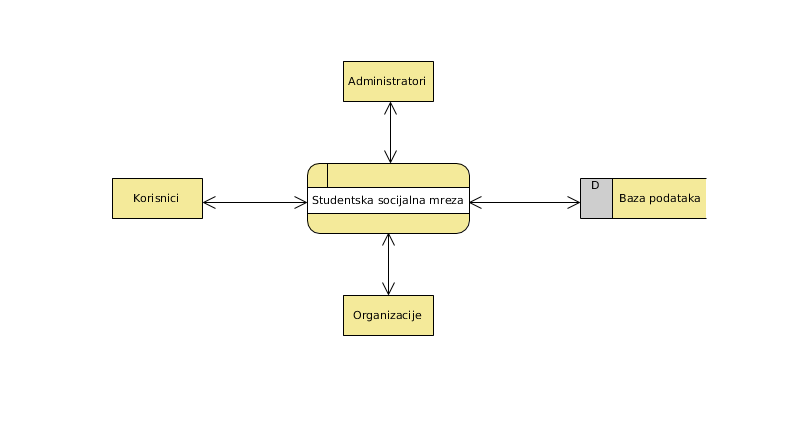
\includegraphics[width=\linewidth]{slike/dijagram_konteksta.png}
    \caption{Dijagram konteksta}
    \label{fig:my_label}
\end{figure}